\chapter{Conclusion}

A novel underwater, open source, and configurable vehicle that can support experiments with both scientific and engineering goals was designed, constructed, and tested in simulation. Propulsion and sensor tests were carried out in a pool, in preparation for autonomy field tests. This final chapter will review the contributions of this thesis and discuss the ongoing and future work. 
% \section{Controller Comparison}
% -practical for use in real life, which control method is better
\section{Contribution}
% What new knowledge was created?
A need for the uDrone was demonstrated. It will allow for greater volumes of coral reef imaging data to be obtained in a safe and reliable manner. Additionally, the uDrone will continue to produce advances in underwater autonomous navigation research from its joint simulation and real world testbed.

This thesis detailed the chosen hardware and software components and explained how they fit together. This system configuration could be used to develop underwater vehicles with similar technical capabilities. 

The mathematical model of the vehicle dynamics will allow for future controller development. Specifically, this work can be used to create a model predictive controller which could greatly improve controllability of the uDrone. 

The two control methods discussed in this document demonstrate how the uDrone navigates through a reef environment. In particular, the code written for the PID controller can be used for future research and development of autonomous controllers.

\section{Ongoing Work}

Work on the uDrone has continued as this thesis drew to a conclusion. This section discusses two areas where work is currently ongoing. 

\subsection{Water Testing}
An initial set of tests has been conducted in a pool. This can be seen in Figure \ref{pool-test} and the video can be viewed at the URL associated with \cite{jd-pool}. The first goal of these tests was to validate the waterproofing of the vehicles. The enclosure and seals are able to seal out water and the electronics were kept dry. The second goal is to test ballasting and buoyancy. The vehicle was very slightly positively buoyant, which is desirable. The center of gravity was slightly below the center of buoyancy, but in the same line. This caused the uDrone to sit horizontally in the water and have a slight moment to keep itself upright in roll, which is ideal. Finally, the vehicle dynamics were tested. This involved manually piloting it around the pool and verifying that it was agile and controllable. While there is no concrete measurement for this, it qualitative performed very well in the water.

\begin{figure}[ht]
    \centering
    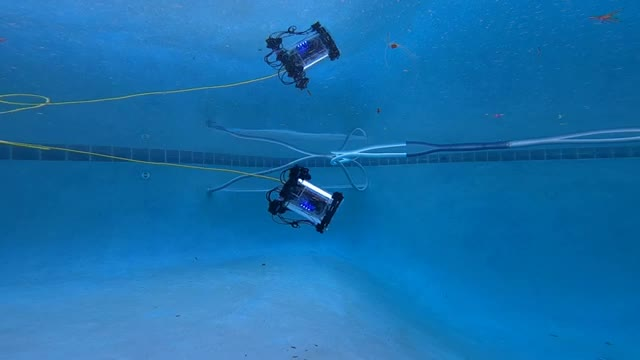
\includegraphics[width=\maxwidth{\textwidth}]{img/pool-test.jpeg}
    \caption{uDrone in the pool during a propulsion test}
    \legend{\emph{Source}: \cite{jd-pool}}
    \label{pool-test}
\end{figure}

\subsection{Diver-Following}

The testbed has allowed for proof of concept tests of vision based navigation. The first of these tests is being run by a DREAMS Lab member and uDrone contributor, A.L.G. Prasad. Using the same PID controller developed as part of this thesis, he was able to write code to enable the uDrone to follow a scuba diver in simulation. This is only the first step in the Vision Based Navigation track, but it is a meaningful step towards autonomy. 

\section{Future Work}\label{future-work}

Despite the achievements laid out here, there is still substantial work that need to be performed for the uDrone to operate in a fully autonomous mode. The two most pressing areas of immediate future work are water tests and vision based navigation.

\subsection{Vision Based Navigation}

The end goal of the uDrone project is for it to be able to navigate unknown environments using vision. This will include aspects of visual-inertial odometry (VIO) and simultaneous localization and mapping (SLAM). Both of these fields are well developed on land but are still emerging in the underwater realm. For example, \cite{mono-vio} developed a method for visual odometer in turbid water using an inexpensive camera. Or, as previously mentioned, \cite{manderson2020visionbased} shows a working application of underwater visual based navigation. Tools and datasets, like AQUALOC, are being created which can aid in the training of vision-based machine-learning algorithms for navigation \parencite{aqualoc}. Underwater visual based navigation is a prime area of research right now and with the uDrone, DREAMS Lab and ASU are well positioned to become contributors and leaders in this area. 

\subsection{Real-World Water Testing}
The next set of pool tests will verify that the uDrone can be autonomously controlled via ROS. Then, once it has been thoroughly tested in a controlled and confined environment, the uDrone will be taken to Hawaii where it will be tested in a real coral environment. The first few tests will include divers following the vehicle to watch for any issues. Eventually, it can complete its first solo autonomous missions.

\subsection{Reinforcement Learning}

With enough trails and data from the real world and an improved simulation it will be possible to create a controller for the uDrone based on reinforcement learning. This has the potential to be both more efficient and more robust than a PID or MPC. This new controller would be trained in simulation using collected data from real world experiments. It may employ other, pre-trained, vision algorithms or be trained as a full end-to-end algorithm. 

\subsection{Hardware Configuration}

Several improvements can already be suggested for the uDrone hardware based on insights yielded from this thesis. Primarily, it was determined that switching the flat front plate of the enclosure to a domed plate would reduce the hydrodynamic drag on the uDrone and allow for the camera to be positioned at different angles. Additionally, more cameras can be added to the body at different angles in order to improve the vision based navigation that will come in the next phase.

In order to continue improving the vehicle configuration, several hardware experiments can be run. The first and most straightforward of these experiments is to test the impact of adjusting the vehicle's ballast. This would allow for different behaviors of the vehicle, which may be desirable for different types of missions. Furthermore, alternative thruster configurations can be tested. For example, if all the thrusters are pitched outward, then the uDrone would have some minimal control authority to move in the Y or Z directions independently of rotating. This would have the drawbacks of being less efficient for motion in the X direction and greatly complicating any models or model based controllers that have been developed. 

%\subsection{Alternative Configurations}
% - Domed front: More hydrodynamics, variable angles of camera
% - Multicamera: Up, Down
% - Thruster Configuration: Tilt out: allow for movement in different directions, move to CB/CG, more hydrobatics

